\documentclass{standalone}
\usepackage{amsmath,amssymb,pgfmath,pgffor,tikz,xifthen}
\usepackage[prefix=M]{xcolor-material}
\usetikzlibrary{calc,decorations.pathmorphing,decorations.pathreplacing,patterns,backgrounds}

\begin{document}

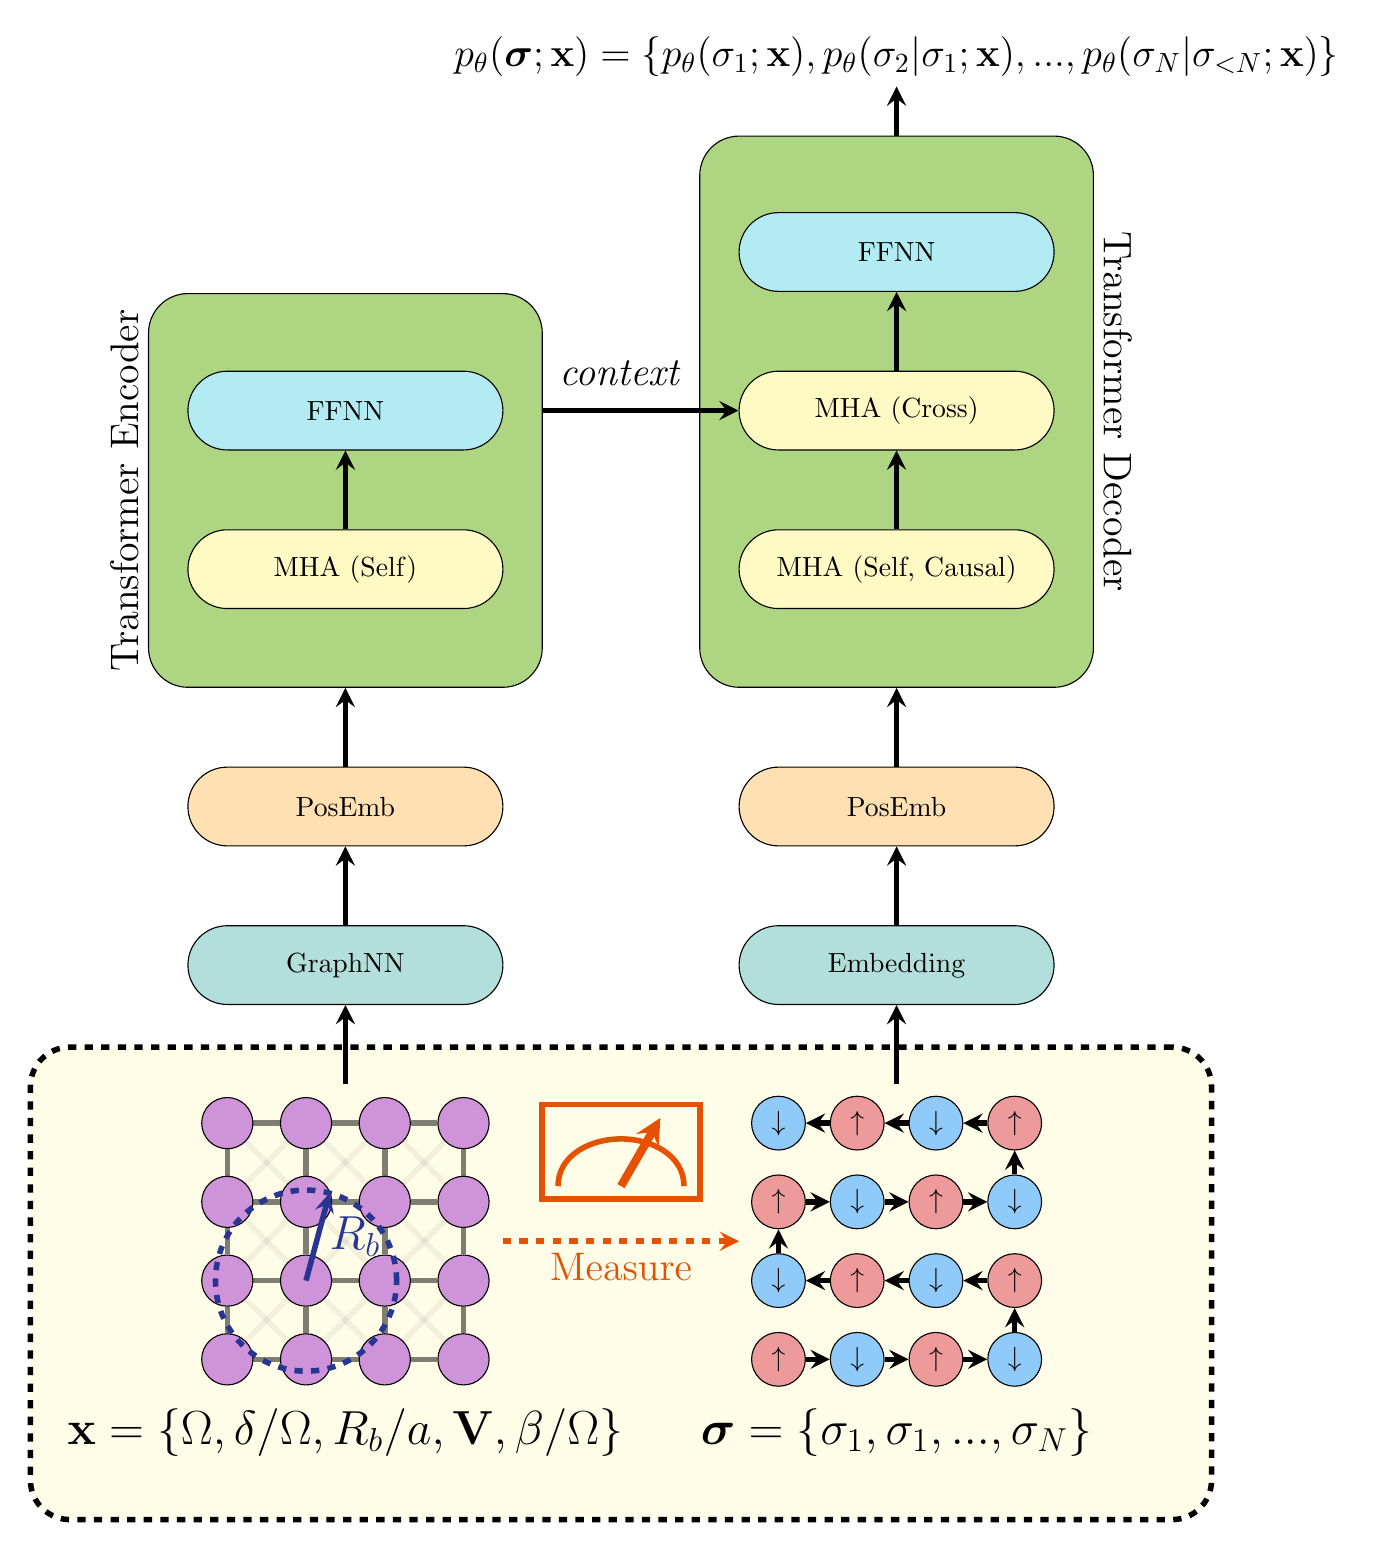
\begin{tikzpicture}

\node [anchor=north, rectangle, fill=MYellow50, draw, dashed, line width=2, rounded corners=0.5cm, minimum height=6cm, minimum width=15cm] (tfdec) at (6,5) {};

%%%%%%%%%%%%%%%%%%%%%%%%%%%%%%%%%%%%%%%%%%%%%%%%%%%%%%%%%%%%%%%%%%%%%%%%%%%%%%%%%%%%%%%

\def\L{4}
\def\Lm{3}

\foreach \i in {1,...,\L} {
\foreach \j in {1,...,\L} {
    \node [circle,fill=MPurple200,draw,minimum size=0.65cm] (spin-\i-\j) at ($(\i,\j) + (0,0)$) {};
}
}

\foreach \i in {1,...,\Lm} {,
\foreach \j in {1,...,\L} {
    \pgfmathsetmacro\ip{int(\i+1)}
    \pgfmathsetmacro\jp{int(\j+1)}
    \draw [-, opacity=0.5, line width = 2] (spin-\i-\j) -- (spin-\ip-\j);
}
}

\foreach \i in {1,...,\L} {
\foreach \j in {1,...,\Lm} {
    \pgfmathsetmacro\ip{int(\i+1)}
    \pgfmathsetmacro\jp{int(\j+1)}
    \draw [-, opacity=0.5, line width = 2] (spin-\i-\j) -- (spin-\i-\jp);
}
}

\foreach \i in {1,...,\Lm} {
\foreach \j in {1,...,\Lm} {
    \pgfmathsetmacro\ip{int(\i+1)}
    \pgfmathsetmacro\jp{int(\j+1)}
    \draw [-, opacity=0.05, line width = 2] (spin-\i-\j) -- (spin-\ip-\jp);
}
}

\foreach \i in {1,...,\Lm} {
\foreach \j in {2,...,\L} {
    \pgfmathsetmacro\ip{int(\i+1)}
    \pgfmathsetmacro\jm{int(\j-1)}
    \draw [-, opacity=0.05, line width=2] (spin-\i-\j) --  (spin-\ip-\jm);
}
}

% \draw [-stealth, line width=2, color=MGreen600] (1,2) --++ (0,1) node [midway, left] {\Large $a$};
\draw [dashed, color=MIndigo800, line width=2] (2,2) circle (1.15cm);
\draw [-stealth, line width=2, color=MIndigo800, rotate around={345:(2,2)}] (2,2) --++ (0,1.15) node [midway, right] {\LARGE $R_b$};

\node [anchor=north] at (\L/2+0.5, 0.5 ) {
\LARGE
$
\mathbf{x} = \{ \Omega, \delta/\Omega, R_b/a, \mathbf{V}, \beta / \Omega \}
$
};

%%%%%%%%%%%%%%%%%%%%%%%%%%%%%%%%%%%%%%%%%%%%%%%%%%%%%%%%%%%%%%%%%%%%%%%%%%%%%%%%%%%%%%%

\foreach \i in {1,...,\L} {
\foreach \j in {1,...,\L} {
    \pgfmathsetmacro\k{int(\i+\L*(\j-1))}
    \pgfmathsetmacro\m{mod(\i+\j,2)}
    \ifthenelse{\equal{\m}{0.0}}{
    \node [circle,fill=MRed200,draw,minimum size=0.65cm] (spin2-\i-\j) at ($(\i,\j) + (7,0)$) {$\uparrow$};
    }
    {
    \node [circle,fill=MBlue200,draw,minimum size=0.65cm] (spin2-\i-\j) at ($(\i,\j) + (7,0)$) {$\downarrow$};
    }
}
}

\foreach \i in {1,...,\Lm} {
\foreach \j in {1,...,\L} {
    \pgfmathsetmacro\ip{int(\i+1)}
    \pgfmathsetmacro\jp{int(\j+1)}
    \pgfmathsetmacro\k{mod(\j,2)}
    \ifthenelse{\equal{\k}{1.0}}{
    \draw [-stealth, line width = 2] (spin2-\i-\j) -- (spin2-\ip-\j);
    }
    {
    \draw [stealth-, line width = 2] (spin2-\i-\j) -- (spin2-\ip-\j);
    }
}
}

\foreach \j in {1,...,\Lm} {
    \pgfmathsetmacro\jp{int(\j+1)}
    \pgfmathsetmacro\ip{int(1 + mod(\j,2)*\Lm)}
    \draw [-stealth, line width = 2] (spin2-\ip-\j) -- (spin2-\ip-\jp);
}

\node [anchor=north] at ($(\L/2+0.5, 0.5) + (7,0)$) {\LARGE $\boldsymbol{\sigma} = \{ \sigma_1,\sigma_1,...,\sigma_N \}$};

%%%%%%%%%%%%%%%%%%%%%%%%%%%%%%%%%%%%%%%%%%%%%%%%%%%%%%%%%%%%%%%%%%%%%%%%%%%%%%%%%%%%%%%

%%%%%%%%%%%%%%%%%%%%%%%%%%%%%%%%%%%%%%%%%%%%%%%%%%%%%%%%%%%%%%%%%%%%%%%%%%%%%%%%%%%%%%%

\coordinate (input1) at (\L/2+0.5,\L+0.5) ;

\node [align=center,anchor=south, rectangle, fill=MTeal100, draw, rounded corners=0.5cm, minimum height=1cm, minimum width=4cm] (enc_graphnn) at ($(input1.north) + (0,1)$) {GraphNN};

\node [align=center,anchor=south, rectangle, fill=MOrange100, draw, rounded corners=0.5cm, minimum height=1cm, minimum width=4cm] (enc_posemb1) at ($(enc_graphnn.north) + (0,1)$) {PosEmb};

\node [align=center,anchor=south, rectangle, fill=MLightGreen300, draw, rounded corners=0.5cm, minimum height=5cm, minimum width=5cm] (tfenc) at ($(enc_posemb1.north) + (0,1)$) {};
\node [anchor=east] at (tfenc.west) {\Large \rotatebox{90}{Transformer Encoder}};

\node [align=center,anchor=south, rectangle, fill=MYellow100, draw, rounded corners=0.5cm, minimum height=1cm, minimum width=4cm] (enc_mha_self) at ($(tfenc.south) + (0,1)$) {MHA (Self)};
\node [align=center,anchor=south, rectangle, fill=MCyan100, draw, rounded corners=0.5cm, minimum height=1cm, minimum width=4cm] (enc_ffnn) at ($(enc_mha_self.north) + (0,1)$) {FFNN};

\draw [-stealth,line width=2] (input1) -- (enc_graphnn);
\draw [-stealth,line width=2] (enc_graphnn) -- (enc_posemb1);
\draw [-stealth,line width=2] (enc_posemb1) -- (tfenc);
\draw [-stealth,line width=2] (enc_mha_self) -- (enc_ffnn);


%%%%%%%%%%%%%%%%%%%%%%%%%%%%%%%%%%%%%%%%%%%%%%%%%%%%%%%%%%%%%%%%%%%%%%%%%%%%%%%%%%%%%%%%


\coordinate (input2) at ($(input1) + (7,0)$);

\node [align=center,anchor=south, rectangle, fill=MTeal100, draw, rounded corners=0.5cm, minimum height=1cm, minimum width=4cm] (dec_emb) at ($(input2.north) + (0,1)$) {Embedding};

\node [align=center,anchor=south, rectangle, fill=MOrange100, draw, rounded corners=0.5cm, minimum height=1cm, minimum width=4cm] (dec_posemb) at ($(dec_emb.north) + (0,1)$) {PosEmb};

\node [align=center,anchor=south, rectangle, fill=MLightGreen300, draw, rounded corners=0.5cm, minimum height=7cm, minimum width=5cm] (tfdec) at ($(dec_posemb.north) + (0,1)$) {};
\node [anchor=west] at (tfdec.east) {\Large \rotatebox{270}{Transformer Decoder}};

\node [align=center,anchor=south, rectangle, fill=MYellow100, draw, rounded corners=0.5cm, minimum height=1cm, minimum width=4cm] (dec_mha_selfcausal) at ($(tfdec.south) + (0,1)$) {MHA (Self, Causal)};
\node [align=center,anchor=south, rectangle, fill=MYellow100, draw, rounded corners=0.5cm, minimum height=1cm, minimum width=4cm] (dec_mha_cross) at ($(dec_mha_selfcausal.north) + (0,1)$) {MHA (Cross)};
\node [align=center,anchor=south, rectangle, fill=MCyan100, draw, rounded corners=0.5cm, minimum height=1cm, minimum width=4cm] (dec_ffnn) at ($(dec_mha_cross.north) + (0,1)$) {FFNN};


\node (output2) at($(tfdec.north) + (0,1)$) {\Large $p_\theta(\boldsymbol{\sigma};\mathbf{x}) = \{ p_\theta(\sigma_1;\mathbf{x}), p_\theta(\sigma_2|\sigma_1;\mathbf{x}),...,p_\theta(\sigma_N|\sigma_{<N};\mathbf{x}) \}$};

\draw [-stealth,line width=2] (input2) -- (dec_emb);
\draw [-stealth,line width=2] (dec_emb) -- (dec_posemb);
\draw [-stealth,line width=2] (dec_posemb) -- (tfdec);
\draw [-stealth,line width=2] (tfdec) -- (output2);
\draw [-stealth,line width=2] (dec_mha_selfcausal) -- (dec_mha_cross);
\draw [-stealth,line width=2] (dec_mha_cross) -- (dec_ffnn);
\draw [-stealth,line width=2] (tfenc.east |- dec_mha_cross.west) -- (dec_mha_cross.west);
\node [anchor=south] at (6,13.25) {\Large \textit{context}};

%%%%%%%%%%%%%%%%%%%%%%%%%%%%%%%%%%%%%%%%%%%%%%%%%%%%%%%%%%%%%%%%%%%%%%%%%%%%%%%%%%%%%%%


\draw [dashed, -stealth, line width=2, color=MOrange900] (4.5,2.5) --++(3, 0) node [midway, below] {\Large Measure};


\node [anchor=south, draw,thick,minimum width=2cm,minimum height=1.2cm, color=MOrange900, line width=2] (rect) at (4.5+1.5,3) {};


\draw [-stealth, color=MOrange900, line width=3, rotate around={330:(6,3+0.2)}] (4.5+1.5,3+0.2) --++ (0,1);

\draw [color=MOrange900, line width=2] (-0.8+6,0.2+3) to[out=90,in=180] (6,0.8+3) to[out=0,in=90] (.8+6,0.2+3);

%%%%%%%%%%%%%%%%%%%%%%%%%%%%%%%%%%%%%%%%%%%%%%%%%%%%%%%%%%%%%%%%%%%%%%%%%%%%%%%%%%%%%%%


\end{tikzpicture}

\end{document}
